% Chapter Template

\chapter{Pilot study} % Main chapter title

\label{Chapter6} % Change X to a consecutive number; for referencing this chapter elsewhere, use \ref{ChapterX}

%----------------------------------------------------------------------------------------
%	SECTION 1
%----------------------------------------------------------------------------------------
The goal of this pilot study is to test if the hypnosis will have any chance of giving any significant results. The pilot study will also test if the tasks in the study actually answers what we want to find out. The pilot study will also give a clearer indication of the limitations of these tests.
\section{Method}
\subsection{Pilot study}
The pilot study was done by showing the test people the developed sketch prototype. Using this sketch prototype the tester sat next to the user and asked them to perform the tasks written down on a piece of paper (In chinese for the Chinese users and in English for the Western users). First the people got a minute to look around the page to get a quick feel for the layout of the site. Then a question was showed to the user and a timer was started at the same time. When the test subject found the requested image or text they indicated that they had found the information and the timer was then stopped. This was repeated until all the tasks where fulfilled.

\section{Results}
The users where asked to perform the following tasks:
\\\\
\textbf{English BBC Questions:}
\begin{enumerate}
	\item Click the news about ivory stabbing
	
	\item Click on the Korean men beauty revolution
	
	\item Click on the news about the freed samung heir
	
	\item Click on the news about Zuma refusing to step down.
	
	\item Click on the news that has to do with a angry sports coach.
	
	\item Click on the long read article about the catholic priest father
	
	\item Click on the video about cooking with strangers
	
	\item Click on the video that has to do with Indonesia

	\item Via the top menu go to the new phones site
	
	\item Via the top menu go to US politics
	
	\item Via the top menu go to news about the stock market
	
\end{enumerate}

\textbf{English QQ Questions}:
\begin{enumerate}

	
	\item Click on the following news: One hundred Hongkong staff more than half hiding in the United States and Canada
	
	\item Click on the following news: Fishermen are no longer allowed to bring their own baits.
	
	\item Click on the following news: Russian fighter pilots last words before blowing himself up with a grenade “For my brothers"
		
	\item Click the following news: True beauty don’t fear wrinkles
		
	\item Click on the video with a Chimpanzee
	
	\item Click on the video below: Premier League - Liverpool 2-2
		
	\item Click on the skyscraper picture
		
	\item Click on the news below: Dow plunge near 700 on Friday what trigged it?
		
	\item Choose from the following menu items: News
		
	\item Choose from the following menu items: Health
		
	\item Choose from the following menu items: Sports
	
	\item Choose from the following menu items: Digital
\end{enumerate}
The BBC pilot study resulted in the following results: 
\begin{figure}[h]
	\centering
	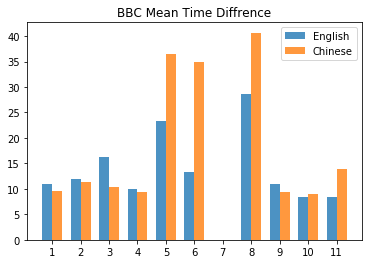
\includegraphics[width=60mm]{Images/pilot_study_bbc_mean_time}
	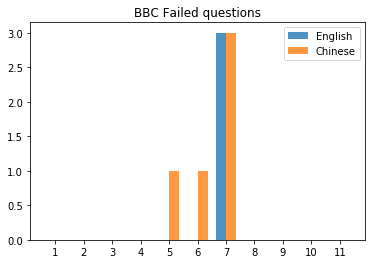
\includegraphics[width=60mm]{Images/pilot_study_bbc_failed}
	\decoRule
		\caption[BBC pilot study results]{Results from the pilot study for the BBC inspired news prototype.}
	\label{fig:pilot_study_bbc}
\end{figure}

The QQ pilot study resulted in the following mean results:
\begin{figure}[h]
	\centering
	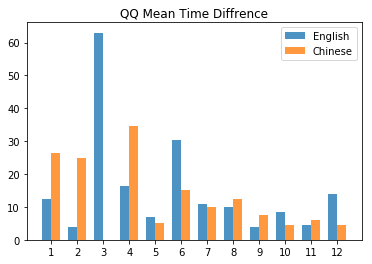
\includegraphics[width=60mm]{Images/pilot_study_qq_mean_time}
	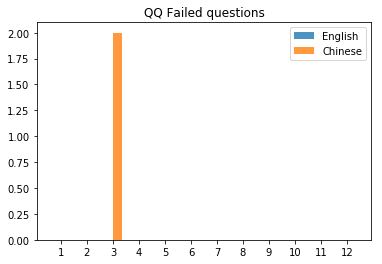
\includegraphics[width=60mm]{Images/pilot_study_qq_failed}
	\decoRule
	\caption[QQ pilot study results]{Results from the pilot study for the QQ inspired news prototype.}
	\label{fig:pilot_study_qq}
\end{figure}

\section{Discussion}
Doing this study provided a lot of relevant information some of the main problems with the test that was identified where that some of the news where repeated on several places of the site this made some tasks irrelevant since the news could be located at several different locations. Some of the questions seemed badly translated as well. For example the question of the sports coach seemed to confuse many of the Chinese users. Also the questions regarding finding images on the qq site did not provide with any meaningful result this since QQ has very few pictures and therefore they did not check how well the user preformed in information dense sites. Another thing that was noticed during the test were how much the positioning of the questions were. The users seem to start their new search pattern from the point of the last task. This means that subjects who were asked to find new information all quickly found news closely located to the previous task. This needs to be kept in mind when designing the next set of questions, it might also be interesting to keep this in mind when analysing the results of the larger study.
\\\\
We can see the measurements from the study in \ref{fig:pilot_study_bbc} and \ref{fig:pilot_study_qq}. Since the goal of the pilot study was to try out if the concept for the real study works we did not have enough participants for this data to have any statistical significance. As mention above the goal of the study was to find problems with the questions, translation and ux. According to (ref vem det nu var) we only need about 5 participants to find the majority of the user experience problems. But if we want this survey to be statistical significant when actually measuring time differences we would need 20 participants on each individual page. This would mean a total of 80 participants.
\\\\
One thing that was noticed that were missing from a usability perspective is asking the user to perform actual tasks. All of the questions where focused on finding information. We would also to some extent test how the users deal with actual tasks and functions that are present on the different sites. One common task that is used on news based sites is giving feedback to the hosts and following the sites on social media.

HMMM TANKAR-------------------
skulle vilja lägga till något som hjälper dig navigera i sidan. så användaren faktist försöker använda det
\section{Conclusion}
Many questions will be changed to better be able to get results for the projects, also both the sites will have questions with the same structure. Both sites will have 20 tasks to perform. Four of the tasks will be about the menu-bar, four of the tasks will be functional, four of the tasks will be about finding precisely described news titles and lastly 4 of the tasks will be about finding more general described news. About half of the tasks will be in the F-shaped pattern view sight. The other half of the questions will be located to the right-hand and central side of the website. Finally the sites will be designed so the content of both sites will be as similar to each other as possible. 

Some functionality will be added to the prototype such as giving feedback and also following on social media. This will be done according to standards as can be seen in \ref{Chapter4}. A menu with the option to give feedback and follow on social media will be added to the right hand side on the Chinese pages respectively on the bottom of the page for the western site.

